\documentclass[a4 paper, 12pt]{article}

\title{DECO2500 - INDIVIDUAL REPORT \\ Feedback 1}
\author{Tean-louise Cunningham (42637460)}
\date{17 April 2020}

\usepackage{geometry}
\geometry{margin=2cm}

\usepackage[utf8]{inputenc}
\usepackage[english]{babel}
\usepackage{xcolor}

\usepackage{appendix}
\usepackage{hyperref}
\hypersetup{
    colorlinks=true,
    linkcolor=black,
    filecolor=black,      
    urlcolor=blue,
}

%\usepackage{standalone}

\setlength{\parindent}{2em}
\setlength{\parskip}{1em}

\usepackage{enumitem}
\setlist{noitemsep, topsep=0pt}
\setlist[enumerate]{parsep=5pt} 

\usepackage{multicol}

% Symbols
\usepackage{amssymb}
%%%%%%%%%%%%%%%%%%%%%%%%%%%%%%%%%%%%%%%%%%
\begin{document}

\section{Iteration 1 - Low Fidelity Prototype}
The initial research and conceptual design of the low-fidelity prototype were previously presented as a \href{run:../MindMap/MindMap.pdf}{mind map} and \href{https://youtu.be/BRX7kF7ynSQ}{presentation}. In review, there are six main features that have been incorporated into the design of the low-fidelity prototype to address users needs. All of these features will be brought to the attention of the user during this first evaluation to determine they align with user needs and whether they should be carried into the next iteration.

    \subsection{Requirements/Conception Design}
    All of these elements of the conceptual design are clearly outlined by the mind map. All important information has been repeated here for easier reference and any recommended revisions from the provided feedback have been applied.
        \subsubsection{System Concept Statement}
        The interaction paradigm is \textbf{mobile} and the interaction mode is \textbf{instructing} only (nudging is simply used as an additional tool for recommendation but is not a mode). As per the feedback, the metaphors used for this application should refer directly to the symbol/real-world representation being used rather than the information they are representing.  
            \begin{multicols}{2}
                \begin{itemize}
                    \item search $\dashrightarrow$ magnifying glass
                    \item arrows 
                    \item bookmark 
                    \item addition $\dashrightarrow$ plus sign
                    \item thumbs up/down 
                    \item tick/cross/question mark 
                    \item filter/settings $\dashrightarrow$ tuning sliders 
                    \item menu
                    \item information $\dashrightarrow$ lower case i 
                    \item account $\dashrightarrow$ person outline 
                    \item map 
                    \item favourite $\dashrightarrow$ heart 
                    \item coupon
                    \item edit $\dashrightarrow$ pencil
                    \item phone
                    \item website $\dashrightarrow$ world
                    \item clock
                    \item address $\dashrightarrow$ Google Maps pin
                    \item navigation $\dashrightarrow$ road sign with arrow
                \end{itemize}
            \end{multicols}

        \subsubsection{Design Principles}
        \begin{multicols}{2}    
            \begin{itemize}
                \item Give clear direction and guidance
                \item Be familiar
                \item Simplify decision process
                \item Encourage collaboration
                \item Maximise customisation opportunities
                \item Open to change
                \item Manageable steps
            \end{itemize}
        \end{multicols}

        \subsubsection{System Requirements}
            \begin{enumerate}
                \item Promote existing deals - Users are informed of whether an option is in their budget.
                \item Interactive Map - Interface needs a way to search for options.
                \item Editable and shareable list - User needs a way to review their options.
                \item Filter menu and map view - Users only want to view what is relevant to their individual needs.
                \item Recommend to a friend - Keep track of user history, remove focus from user reviews.      
                \item Restaurant information - Information to make an informed decision.
            \end{enumerate}   


    \subsection{Low Fidelity Prototype}
    Below is the proposed low fidelity prototype as submitted with the mind map. 
    \begin{figure} [H]
        \centering
        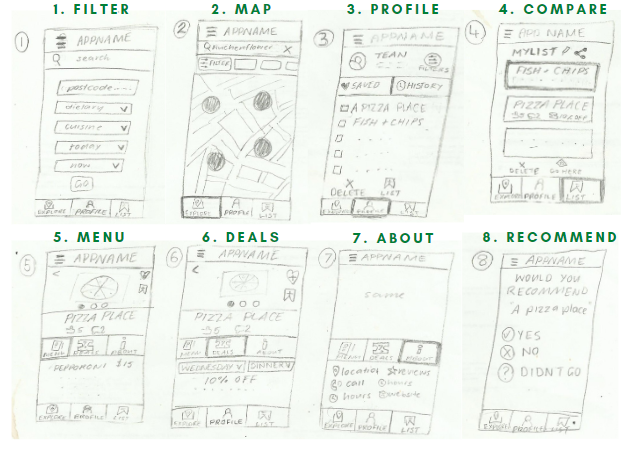
\includegraphics[width=\textwidth, frame]
            {./Low_Fidelity/Low_Prototype.PNG} 
        \caption{Low Prototype}
    \end{figure}  
    
    
% 3.1.1 Low Fidelity Prototype Evaluation
\subsection{Low Fidelity Prototype Evaluation}

\subsubsection{Evaluation Methods}
The purpose of these evaluations is to learn more about the users' needs, confirm that the conceptual model is appropriate for the users, and to provide feedback about design and flow. It is imperative that any misalignment of values or expectations are identified at this early stage before further time is spent on interaction design. Users must be able to understand how the system works and it must align with their expectations to be a worthwhile project [Studio 4 Week 5]. The evaluation method chosen for the Low Fidelity Prototype is a combination of Design Walkthrough, Co-design and Technology Acceptance Model (TAM).

A design walkthrough involves giving the user a task and, without guidance, ask them to complete the task. By observing and documenting how they interact with the system, feedback on how users expect the system to operate and what they they expect the system can be obtained [32]. This feedback provides clearly whether the conceptual model chosen is appropriate to the users mental model [31, 37]. This method was chosen as the steps involved in using the application are almost the same for every instance, and so it is imperative that users are able to easily complete these steps (i.e the task) without cognitive overload at this early stage of design [30, 38].

The co-design process generally involves explaining to the user how the system works and asking for their opinion how they would design the features of the application (Evaluation Guide). For this evaluation, at points during the design walkthrough when a user gets stuck, in addition to asking them what the issues are and what they are experiencing, additional co-design practices will be adopted. This includes asking the user what they think should be happening and how they would design this part to be more intuitive [31]. Since the user is in control of instructing the system it is important that they are able to achieve their goal of choosing a place to dine out the way they want to and expect, especially since it is a process that will be repeated on average twice a week for them [50]. 

TAM consists of a set of questions based on perceived usefulness, perceived ease of use, attitude and intention to use the system. These questions are scaled from 1 (strongly disagree) to 4 (strongly agree). For this evaluation, eight of the questions were selected (at least one from each category). These questions were identified as most relatable to the purpose of the application, without being repetitive. The questions provide quantitative analysis that can assist with identifying problem areas of user acceptance, however by themselves they don't provide the reasoning behind the response [32]. So in addition to these questions, follow up questions will be asked when a response less than strongly agree is selected to gain further insight into the users experience to understand why there is a gap between mental models [31, 37]. This method was incorporated as an extension to the design walkthrough/co-design process to determine whether users could not only use the system but whether they accept it and believe the design and the features assist them with mitigating the problem of deciding where to dine out [39].

Together these evaluation methods provide a succinct overview of whether at this stage of design that application gives the user what they want, what gaps may exist in the conceptual model and the overall acceptance of the design and flow of the prototype.

\subsubsection{Evaluation Protocol}
This protocol was created to provide structure and consistency amongst evaluation of participants. The protocol outlines the flow of the evaluation including scripts, instructions and details of notes to be taken [31, 32]. The protocol can be viewed as \hyperref[sec:A.1]{Appendix A.1}. Due to current measures relating to COVID-19 all evaluations were performed online, unless part of the family unit. Users are invited to a Google Form where they are asked to sign in with their Google Account. From here they can navigate themselves through all aspects of the evaluation. The form can be viewed in \hyperref[sec:A.2]{Appendix A.2}.  

Firstly, the user is introduced to the evaluation process and asked to complete a consent form online. The consent form is then uploaded in the provided section on the form. Secondly, the user is given instructions for the Design Walkthrough and directed, via a link, to a Google Slides presentation. Here they are given the task and access to navigate through slides depicting different pages of the paper prototype. The task is fairly vague to provide feedback on whether it is clear to the users what features are available without being told. The presentation is designed so that when users select areas of the paper prototype that are ‘clickable’ they are directed to the appropriate slide with the corresponding page. The presentation can be viewed in \hyperref[sec:A.3]{Appendix A.3.}

Thirdly, whilst completing the task any time they are stuck for a period of time they are asked to stop and follow up questions are asked, including contribution of design as part of the co-design process. Finally, once the user has completed the task they select a link on the presentation that takes them back to the Google Form where they will complete the TAM evaluation. On the form, users will select their answer between 1 and 4 (strongly agree) which will be stored as quantitative results and follow up questions will be asked for further clarification. The results can be viewed in \hyperref[sec:A.4]{Appendix A.4}. Throughout all sections of this process, notes were taken of observations and feedback. These notes can be seen in \hyperref[sec:A.5]{Appendix A.5}.

\subsubsection{Evaluation Results}
The following provides an overview of the results and feedback from the evaluations and is separated by the key features of the application.

\begin{enumerate}
    \item Filter by preferences (including both craving and dietary requirements) - this filtering extends to the map results and menu display
        \begin{itemize}
            \item Users liked that they had the option to filter by dietary and cuisine. 
            \item Some confusion about the difference between cuisine and dietary which would be clear when the dropdowns are clickable.
            \item It wasn't clear that the menu was filtered as well, users noted that if they had been able to filter they probably would have noticed that it was only showing specific meals.
            \item A user wanted to be able to view other menu items as well and suggested that below the filtered items on the menu page there was also a way to access the full menu or change filters on this page. 
        \end{itemize}

    \item Interactive map - replicate the familiar experience of exploring destinations
        \begin{itemize}
            \item Users had no problem selecting a restaurant
            \item About half of the users selected the filter icon before picking a restaurant. They either expected to be taken back to the preference page or bring up a more detailed version of the same list (with those previously chosen pre-selected). 
        \end{itemize}

    \item Promote existing deals - have existing deals from restaurants separate from the menu and easily viewable based on date selection
        \begin{itemize}
            \item Users liked that deals was easily accessible and was one of the main tabs on the restaurant page. 
            \item Was clear that it was filtered based on the day and that they could change that selection in this tab.
        \end{itemize}

    \item Editable and shareable list - provide support to be able to compare options and share these with others
        \begin{itemize}
             
            \item For most users, when they reached the restaurant page it was not clear what the next step was. They looked at all the information and most got stuck.
            \item Most users didn't notice the small list icons in the corner. Their attention was on the six main tabs. When asked whether this was a good position for these icons all but 1 users said yes if it was clearer what the list was.
            \item Many of the users didn't recognise what the 'list' icon was. One of the suggestion was to add the text 'Add to list' and another was to change the icon to scales (the icon would also change on the main tab). 
            \item Many of the users mentioned that before getting to the list page they didn't know what the 'list' icon on main tab meant. Once reaching the list page, for some it wasn't clear whether it was a list for them to compare or a list of places they have saved for later.  One of the suggestions was a different name, such as 'Compare' since 'list' was vague. Also, a design suggestion was to use scales as the icon. 
            \item Most of the users noticed the share button and knew exactly what it did, one of the users suggested adding the text 'share' as well like every other icon  
            \item The delete, edit and go here icons were all clear. Users liked that you could just be directed straight there after deciding. 
            \item Once on the list page, most users were happy to just select a restaurant and go there as currently designed. They were happy with just have the name, rating and deals information.
        \end{itemize}

    \item Recommend to a friend - focus on word-of-mouth recommendations instead of star ratings
        \begin{itemize}
            \item Users liked the idea reviews were friends only. In the TAM evaluation when asking if they would recommend, some commented that this would mean they had a better experience on the app. 
            \item Users understood the thumbs up and down was ratings, but not that it was friends only until it was explained.
            \item None of the users had issues with the notification page, and understood it was related to friend recommendations (after being told earlier). Like the clear wording and only 3 options. 
            \item Users liked that they would be nudged later without having to remember to go back and do it themselves later, especially since the more people that reviewed the better the ratings.
            \item One of the users wanted to be able to see other reviews too and raised the questions 'What if I don't have friends/know people who live in my area?'. They saw the star ratings on the information page, but wanted to see others thumbs up and down recommendation. They suggested that on the restaurant page where the icons are to have with the default as friends and swipe to be able to see all reviews from the app.
        \end{itemize}

    \item Restaurant information - ensure users are able to readily access general information about a restaurant without being overwhelmed 
        \begin{itemize} 
            \item Users understood all of the icons on the about page, liked that this was one of the tabs but not the first one.  
            \item Users had no issues with finding the information about the restaurants.
            \item Once on the list page, some of the users expected to be able to select the restaurant and be taken back to the restaurant page or see more information. One suggestion was to incorporate right and left swiping for different actions. Another suggestion, from a user who wanted to be able to call the place, suggested when selecting a restaurant it overshadowed the name and you had the icons for delete, more information, call and directions.  
        \end{itemize}
\end{enumerate}


\subsubsection{Evaluation Analysis}
From the process of this evaluation, there are a number of key factors that will influence the design of the medium prototype to ensure increased usability and acceptance of the application for the user. For users deciding where to dine out, this prototype has met their needs. From the walkthrough aspect of the evaluation, all users interacted with all of the features of the system, with the list feature the only aspect that needed guidance to reach. On the TAM evaluation, the overwhelming result for the perceived usefulness of the app was strongly agree. Users said they felt all aspects of the application were important in assisting them and especially liked the simpler rating system from friends and the ease of deal access. Therefore, all features of the low fidelity prototype will be carried through to the next iteration.

From the evaluations it is evident that specific areas of the conceptual model didn't match the users mental models [29, 37]. The results of the TAM evaluation showed that the areas of concern were perceived ease of use and attitude. For all users there was only one area of the application in which they had concerns. For some, this was during the gulf of execution due to the misunderstanding of how to to complete the task, that is not knowing how or that they could proceed from the restaurant page to the list page. For others, this was during the gulf of evaluation, as there was the misalignment of design expectation of selecting a restaurant on the list page before proceeding to the location [28, 36]. During the TAM follow up questions users said they would rate strongly agree in these categories if their suggestions from the co-design were adopted. 

Overall, users had no feedback about the overall flow of the application. During the walkthrough, users appreciated the simple design and all commented on the three tabs used to break up the restaurant page as sleek, and easy to use and understand. Most of the icons were recognisable by users, who especially liked when there was text accompanying them. For the next iteration, using the suggestions from the co-design the metaphor used for the list will instead be scales, accompanied by the new name of 'compare'. Additionally, on the list page, when selecting a restaurant an overshadow of icons with text will appear showing the existing delete and go here icons as well as more info and call. Not only does this make it clear what selecting the restaurant does and allow them to instruct the system as they want, but also saves screen real estate and uses Fitts Law to reduce cognitive load [40, 53].  

\end{document}